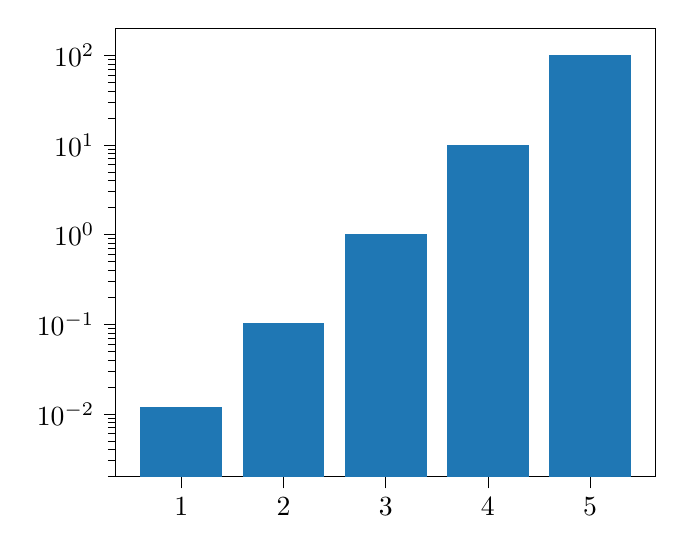
\begin{tikzpicture}

\definecolor{darkgray176}{RGB}{176,176,176}
\definecolor{steelblue31119180}{RGB}{31,119,180}

\begin{axis}[
log basis y={10},
tick align=outside,
tick pos=left,
x grid style={darkgray176},
xmin=0.36, xmax=5.64,
xtick style={color=black},
y grid style={darkgray176},
ymin=0.002, ymax=200,
ymode=log,
ytick style={color=black}
]
\draw[draw=none,fill=steelblue31119180] (axis cs:0.6,0.002) rectangle (axis cs:1.4,0.012);
\draw[draw=none,fill=steelblue31119180] (axis cs:1.6,0.002) rectangle (axis cs:2.4,0.102);
\draw[draw=none,fill=steelblue31119180] (axis cs:2.6,0.002) rectangle (axis cs:3.4,1.002);
\draw[draw=none,fill=steelblue31119180] (axis cs:3.6,0.002) rectangle (axis cs:4.4,10.002);
\draw[draw=none,fill=steelblue31119180] (axis cs:4.6,0.002) rectangle (axis cs:5.4,100.002);
\end{axis}

\end{tikzpicture}
